\documentclass[border=6pt,tikz]{standalone}
\usepackage{amsmath,amssymb}
\usepackage{tikz}
\usetikzlibrary{arrows.meta,calc,decorations.pathreplacing,patterns,shapes.geometric,positioning,shadings,plotmarks}

\begin{document}
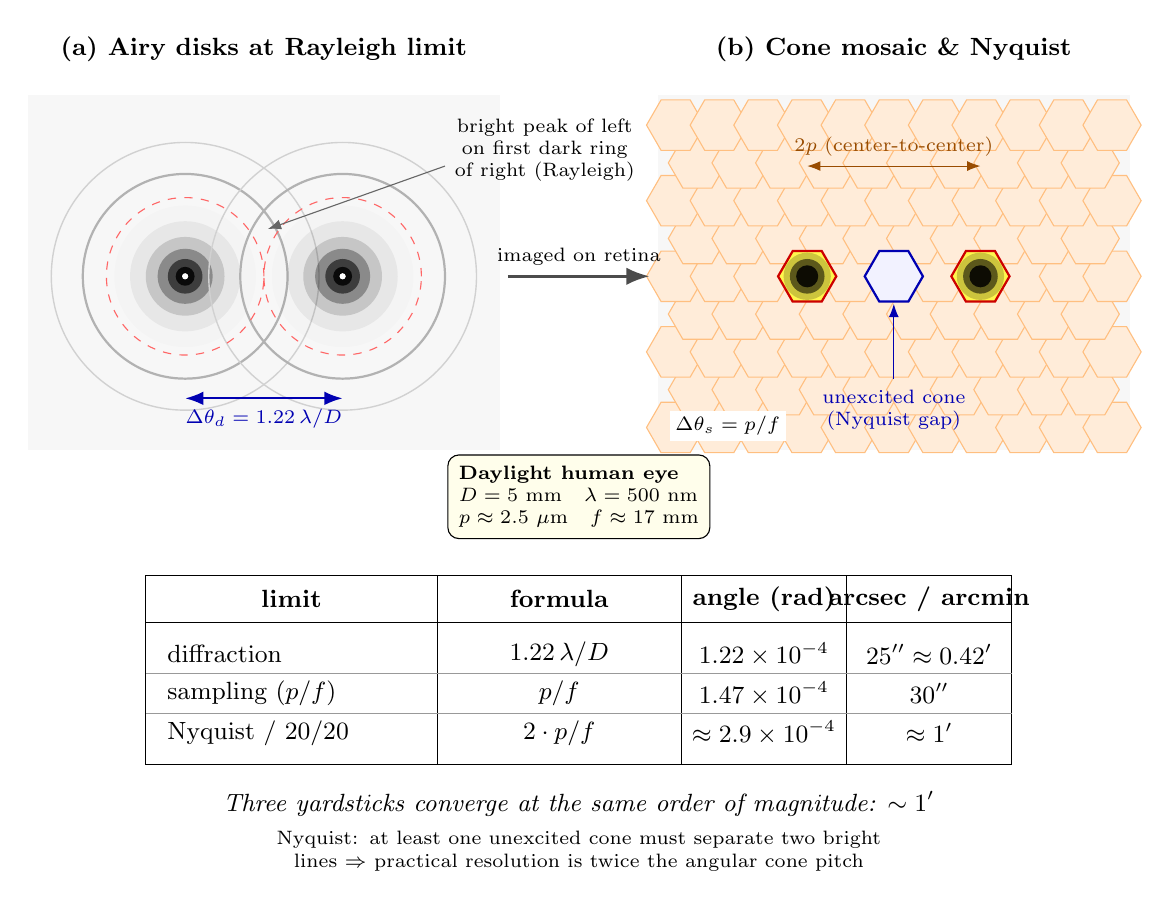
\begin{tikzpicture}[>=Latex,font=\sffamily\small]

% =====================================================================
% TOP-LEFT PANEL: Two Airy disks at Rayleigh separation
% =====================================================================
% Coordinate center (0,0); Airy disk with first dark ring at r=1
% Two disks centered at (-1,0) and (+1,0), so that bright spot of one
% sits on first dark ring of the other.

\begin{scope}[shift={(0,6)}]

% Panel title
\node[font=\small\bfseries,anchor=south] at (0,2.6)
  {(a) Airy disks at Rayleigh limit};

% Background rectangle
\fill[black!3] (-3,-2.2) rectangle (3,2.3);

% --- Airy disk at (-1,0) ---
% Intensity ~ exp(-3 r^2) + very weak first bright ring at r=1.3
% Use concentric shaded rings to suggest Airy pattern
\foreach \r/\op in {0.05/100,0.12/80,0.22/55,0.35/30,0.5/14,0.7/5,0.9/1}{
  \fill[black,opacity=\op/100] (-1,0) circle (\r);
}
% Airy: first bright ring (faint) around r=1.2-1.4
\draw[black!30,line width=0.8pt] (-1,0) circle (1.3);
\draw[black!18,line width=0.5pt] (-1,0) circle (1.7);

% --- Airy disk at (+1,0) ---
\foreach \r/\op in {0.05/100,0.12/80,0.22/55,0.35/30,0.5/14,0.7/5,0.9/1}{
  \fill[black,opacity=\op/100] (1,0) circle (\r);
}
\draw[black!30,line width=0.8pt] (1,0) circle (1.3);
\draw[black!18,line width=0.5pt] (1,0) circle (1.7);

% First dark ring (radius = 1) drawn as dashed circle for each
\draw[red!60,dashed,line width=0.4pt] (-1,0) circle (1);
\draw[red!60,dashed,line width=0.4pt] (1,0) circle (1);

% Centers marked
\fill[white] (-1,0) circle (0.04);
\fill[white] (1,0) circle (0.04);

% Arrow indicating Delta theta
\draw[<->,thick,blue!70!black] (-1,-1.55) -- (1,-1.55)
  node[midway,below,font=\scriptsize,blue!70!black]
  {$\Delta\theta_d = 1.22\,\lambda/D$};

% Annotation of "center falls on first dark ring"
\draw[->,>=Latex,thin,black!60] (2.3,1.4) -- (0.05,0.6);
\node[font=\scriptsize,align=center,anchor=west] at (2.3,1.6)
  {bright peak of left\\on first dark ring\\of right (Rayleigh)};

\end{scope}

% =====================================================================
% TOP-RIGHT PANEL: Hexagonal cone mosaic with two imaged spots
% =====================================================================
\begin{scope}[shift={(8,6)}]

% Panel title
\node[font=\small\bfseries,anchor=south] at (0,2.6)
  {(b) Cone mosaic \& Nyquist};

% Background
\fill[black!3] (-3,-2.2) rectangle (3,2.3);

% Hexagonal cone mosaic
% Hex side s, so horizontal spacing = sqrt(3)*s, vertical = 1.5*s
% We pick s = 0.32 so that center-to-center spacing = sqrt(3)*0.32 ~ 0.55
\def\hs{0.32}

% Draw hex grid: rows i from -4..4, cols j from -5..5
\foreach \i in {-4,-3,-2,-1,0,1,2,3,4}{
  \foreach \j in {-5,-4,-3,-2,-1,0,1,2,3,4,5}{
    \pgfmathsetmacro{\cx}{\j*1.732*\hs + mod(abs(\i),2)*0.866*\hs}
    \pgfmathsetmacro{\cy}{\i*1.5*\hs}
    \pgfmathparse{(\cx>-2.9) && (\cx<2.9) && (\cy>-2.0) && (\cy<2.05)}
    \ifnum\pgfmathresult=1
      \node[regular polygon,regular polygon sides=6,
            draw=orange!50,fill=orange!15,minimum size=\hs*2*1.155 cm,
            inner sep=0,line width=0.4pt,rotate=0]
        at (\cx,\cy){};
    \fi
  }
}

% Highlight two "lit" cones (excited by the two Airy bright spots)
% Spots at horizontal separation ~2*hs*sqrt(3) ~ 1.1 cm,
% with one UNEXCITED cone in between (Nyquist).
% Place bright spots at x = -1.1 and x = +1.1, y = 0
\node[regular polygon,regular polygon sides=6,
      draw=red!80!black,fill=yellow!70,minimum size=\hs*2*1.155 cm,
      inner sep=0,line width=0.8pt]
  at (-1.1,0){};
\node[regular polygon,regular polygon sides=6,
      draw=red!80!black,fill=yellow!70,minimum size=\hs*2*1.155 cm,
      inner sep=0,line width=0.8pt]
  at (1.1,0){};

% Middle (unexcited) cone highlighted with thick border
\node[regular polygon,regular polygon sides=6,
      draw=blue!70!black,fill=blue!5,minimum size=\hs*2*1.155 cm,
      inner sep=0,line width=0.8pt]
  at (0,0){};

% Imaged Airy spots (small gradient dots) on the two excited cones
\fill[black,opacity=0.85] (-1.1,0) circle (0.14);
\fill[black,opacity=0.55] (-1.1,0) circle (0.22);
\fill[black,opacity=0.20] (-1.1,0) circle (0.3);
\fill[black,opacity=0.85] (1.1,0) circle (0.14);
\fill[black,opacity=0.55] (1.1,0) circle (0.22);
\fill[black,opacity=0.20] (1.1,0) circle (0.3);

% Annotation: "unexcited" cone
\draw[->,>=Latex,thin,blue!70!black] (0,-1.3) -- (0,-0.35);
\node[font=\scriptsize,blue!70!black,align=center] at (0,-1.7)
  {unexcited cone\\(Nyquist gap)};

% Scale bar for cone spacing p
\draw[<->,thin,orange!60!black] (-1.1,1.4) -- (1.1,1.4);
\node[font=\scriptsize,orange!60!black,above] at (0,1.4)
  {$2p$ (center-to-center)};

% sampling-limit formula
\node[font=\scriptsize,anchor=south west,fill=white,inner sep=2pt]
  at (-2.85,-2.1) {$\Delta\theta_s = p/f$};

\end{scope}

% =====================================================================
% CONNECTING ARROW: from Airy panel to cone panel
% =====================================================================
\draw[->,>=Latex,very thick,gray!60!black]
  (3.1,6) -- (4.9,6)
  node[midway,above,font=\scriptsize,black]
  {imaged on retina};

% =====================================================================
% PARAMETER BOX
% =====================================================================
\node[draw,rounded corners,fill=yellow!8,font=\scriptsize,
      align=left,inner sep=4pt]
  at (4,3.2)
  {\textbf{Daylight human eye}\\
   $D = 5$ mm\quad $\lambda = 500$ nm\\
   $p \approx 2.5\ \mu$m\quad $f \approx 17$ mm};

% =====================================================================
% COMPARISON TABLE (bottom)
% =====================================================================
\begin{scope}[shift={(0,0)}]

% Outer frame
\draw[black,thin] (-1.5,-0.2) rectangle (9.5,2.2);

% Header row
\draw[black,thin] (-1.5,1.6) -- (9.5,1.6);
% Column separators
\draw[black,thin] (2.2,-0.2) -- (2.2,2.2);
\draw[black,thin] (5.3,-0.2) -- (5.3,2.2);
\draw[black,thin] (7.4,-0.2) -- (7.4,2.2);

% Header text
\node[font=\small\bfseries] at (0.35,1.9) {limit};
\node[font=\small\bfseries] at (3.75,1.9) {formula};
\node[font=\small\bfseries] at (6.35,1.9) {angle (rad)};
\node[font=\small\bfseries] at (8.45,1.9) {arcsec / arcmin};

% Row 1: diffraction
\node[font=\small,anchor=west] at (-1.35,1.2) {diffraction};
\node[font=\small] at (3.75,1.2) {$1.22\,\lambda/D$};
\node[font=\small] at (6.35,1.2) {$1.22 \times 10^{-4}$};
\node[font=\small] at (8.45,1.2) {$25'' \approx 0.42'$};

% Row 2: sampling (angular cone)
\node[font=\small,anchor=west] at (-1.35,0.7) {sampling ($p/f$)};
\node[font=\small] at (3.75,0.7) {$p/f$};
\node[font=\small] at (6.35,0.7) {$1.47 \times 10^{-4}$};
\node[font=\small] at (8.45,0.7) {$30''$};

% Row 3: Nyquist / 20/20
\node[font=\small,anchor=west] at (-1.35,0.2) {Nyquist / 20/20};
\node[font=\small] at (3.75,0.2) {$2 \cdot p/f$};
\node[font=\small] at (6.35,0.2) {$\approx 2.9 \times 10^{-4}$};
\node[font=\small] at (8.45,0.2) {$\approx 1'$};

% Row separators
\draw[black!40,thin] (-1.5,0.95) -- (9.5,0.95);
\draw[black!40,thin] (-1.5,0.45) -- (9.5,0.45);

\end{scope}

% Table caption
\node[font=\small\itshape] at (4,-0.7)
  {Three yardsticks converge at the same order of magnitude: $\sim 1'$};

% Nyquist annotation
\node[font=\scriptsize,align=center,text width=8cm] at (4,-1.3)
  {Nyquist: at least one unexcited cone must separate two bright lines
   $\Rightarrow$ practical resolution is twice the angular cone pitch};

\end{tikzpicture}
\end{document}
